\documentclass[10pt]{beamer}
\mode<presentation>{\usetheme{Madrid}}

\usepackage{graphicx} 
\usepackage{booktabs}
\usepackage{blindtext}


\title[Short title]{Full Title} 

\author{Nils}
\institute[UZH]
{
University of Zurich}
\date{\today}

\begin{document}


\begin{frame}
\titlepage
\end{frame}


\begin{frame}
\frametitle{Titel}
\end{frame}


\begin{frame}
\frametitle{abc}
\begin{itemize}
\item Lorem ipsum dolor sit amet, consectetur adipiscing elit
\item Aliquam blandit faucibus nisi, sit amet dapibus enim tempus eu
\item Nulla commodo, erat quis gravida posuere, elit lacus lobortis est, quis porttitor odio mauris at libero
\item Nam cursus est eget velit posuere pellentesque
\item Vestibulum faucibus velit a augue condimentum quis convallis nulla gravida
\end{itemize}
\end{frame}


\begin{frame}
\frametitle{def}
\end{frame}

\begin{frame}
\frametitle{theorem}
\begin{theorem}
	Let \(f\) be a function whose derivative exists in every point, then \(f\) 
is a continuous function.
\end{theorem}

\end{frame}


\begin{frame}
\frametitle {this is a table}
\begin{table}
	\centering
	\caption{total non-financial debt as percentage of GDP}
	\begin{tabular}{l|rrr|rr}
		\midrule
		\multicolumn{1}{r}{} & \multicolumn{3}{c|}{Levels} & \multicolumn{2}{c}{Changes} \\
		\cmidrule{2-6}    \multicolumn{1}{r}{} & \multicolumn{1}{c}{2000} & \multicolumn{1}{c}{2010} & \multicolumn{1}{c|}{2019} & \multicolumn{1}{c}{2000-10} & \multicolumn{1}{c}{2010-19} \\
		\midrule
		Switzerland & 241   & 243   & 284   & 2     & 41 \\
		United States & 186   & 250   & 250   & 65    & 0 \\
		Germany & 187   & 199   & 181   & 12    & -18 \\
		Norway & 184   & 270   & 270   & 86    & 0 \\
		France & 197   & 266   & 329   & 69    & 63 \\
		Austria & 196   & 238   & 226   & 42    & -12 \\
		Australia & 154   & 204   & 236   & 50    & 32 \\
		Spain & 173   & 285   & 268   & 112   & -17 \\
		Sweden & 201   & 269   & 289   & 68    & 20 \\
		Japan & 313   & 342   & 380   & 29    & 38 \\
		Italy & 192   & 248   & 258   & 56    & 10 \\
		United Kingdom & 180   & 267   & 275   & 87    & 8 \\
		\midrule
		Advanced Economies\footnotemark[2] & 212   & 254   & 272   & 42    & 18 \\
			\end{tabular}%
	\label{tab:total non financial debt as percentage of GDP}%
\end{table}%

\end{frame}



\begin{frame}
\frametitle{this is a figure}

\begin{figure}[h]
	\centering
	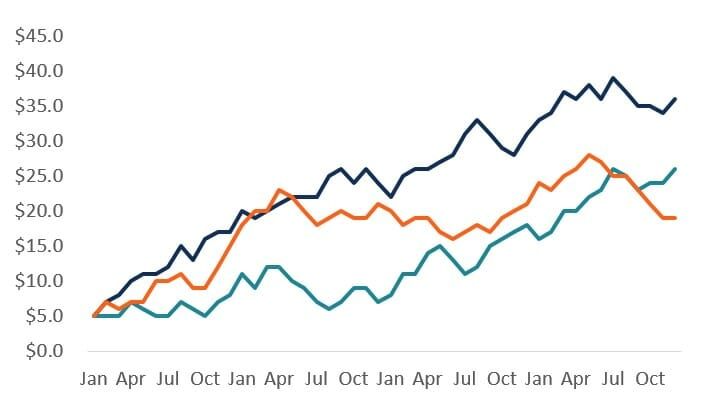
\includegraphics[width=0.9\textwidth]{line-graph.jpg}
	\caption{line graph}
	{Source: Web}
	\label{fig:basicgrowthreg}
\end{figure}

\end{frame}




\end{document}